% CVPR 2024 Paper Template; see https://github.com/cvpr-org/author-kit

\documentclass[10pt,twocolumn,letterpaper]{article}

%%%%%%%%% PAPER TYPE  - PLEASE UPDATE FOR FINAL VERSION
\usepackage{cvpr}              % To produce the CAMERA-READY version
%\usepackage[review]{cvpr}      % To produce the REVIEW version
%\usepackage[pagenumbers]{cvpr} % To force page numbers, e.g. for an arXiv version
\usepackage{diagbox}
\usepackage{graphicx}
\usepackage{amsmath}
\usepackage{amssymb}
\usepackage{booktabs}
\usepackage[dvipsnames]{xcolor}
\usepackage{flexisym}
\usepackage{amsmath}
\usepackage{multirow}
\usepackage{tabularx}
\usepackage{enumitem}

\usepackage{amssymb}% http://ctan.org/pkg/amssymb
\usepackage{pifont}% http://ctan.org/pkg/pifont
\newcommand{\cmark}{\ding{51}}%
\newcommand{\xmark}{\ding{55}}%

% Import additional packages in the preamble file, before hyperref
% Copied & adapted from
% https://github.com/dustinvtran/latex-templates/blob/master/papers/preamble/preamble.tex


\usepackage{amsmath, amssymb, amsthm}
\usepackage{mathtools}
\usepackage{bbm}
\usepackage{dsfont}


\usepackage[usenames,dvipsnames]{xcolor}
\newcommand{\red}[1]{\textcolor{BrickRed}{#1}}
\newcommand{\orange}[1]{\textcolor{BurntOrange}{#1}}
\newcommand{\green}[1]{\textcolor{OliveGreen}{#1}}
\newcommand{\blue}[1]{\textcolor{NavyBlue}{#1}}
\newcommand{\sky}[1]{\textcolor{SkyBlue}{#1}}
\newcommand{\gray}[1]{\textcolor{black!60}{#1}}

% # COUNTERS

\renewcommand{\labelenumi}{\color{black!67}{\arabic{enumi}.}}
\renewcommand{\labelenumii}{{\color{black!67}(\alph{enumii})}}
\renewcommand{\labelitemi}{{\color{black!67}\textbullet}}

% # FIGURES

\usepackage{graphicx}
\usepackage[labelfont=bf]{caption}
\usepackage[format=hang]{subcaption}

% # TABLES

\usepackage{booktabs, array}
\usepackage{multirow}

% # ALGORITHMS

\usepackage[algoruled]{algorithm2e}
\setlength{\interspacetitleruled}{8pt}
\usepackage{listings}
\usepackage{fancyvrb}
\fvset{fontsize=\small}

% # BIBLIOGRAPHY AND LINKS

\usepackage{natbib}
\bibliographystyle{abbrvnat}
\usepackage[colorlinks,linktoc=all,pagebackref=true]{hyperref}
\usepackage[hypcap=true]{caption}
\hypersetup{citecolor=NavyBlue}
\hypersetup{linkcolor=NavyBlue}
\hypersetup{urlcolor=NavyBlue}
\usepackage[nameinlink,capitalise]{cleveref}
\creflabelformat{equation}{#2\textup{#1}#3}  % <- remove parenthesis from equations

% # CODE SNIPPETS

\lstdefinestyle{mystyle}{
    commentstyle=\color{OliveGreen},
    numberstyle=\tiny\color{black!60},
    stringstyle=\color{BrickRed},
    basicstyle=\ttfamily\scriptsize,
    breakatwhitespace=false,
    breaklines=true,
    captionpos=b,
    keepspaces=true,
    numbers=none,
    numbersep=5pt,
    showspaces=false,
    showstringspaces=false,
    showtabs=false,
    tabsize=2
}
\lstset{style=mystyle}

\newsavebox\CBox 
\newcommand{\spm}[1]{\scriptstyle{\pm#1}}
\def\textBF#1{\sbox\CBox{#1}\resizebox{\wd\CBox}{\ht\CBox}{\textbf{#1}}}

% # ACRONYMS
\usepackage[acronym,nowarn,section,nogroupskip,nonumberlist]{glossaries}
\glsdisablehyper{}

\newacronym[\glslongpluralkey={Gaussian Processes}]{gp}{\textsc{gp}}{Gaussian Process}
\newacronym[\glslongpluralkey={Conditional Neural Processes}]{cnp}{\textsc{cnp}}{Conditional Neural Process}
\newacronym[\glslongpluralkey={Neural Processes}]{np}{\textsc{np}}{Neural Process}
\newacronym[\glslongpluralkey={Neural Process Families}]{npf}{\textsc{npf}}{Neural Process Family}
\newacronym[\glslongpluralkey={Attentive Neural Processes}]{anp}{\textsc{anp}}{Attentive Neural Process}
\newacronym[\glslongpluralkey={Conditional Attentive Neural Processes}]{canp}{\textsc{canp}}{Conditional Attentive Neural Process}
\newacronym[\glslongpluralkey={Convolutional Conditional Neural Processes}]{convcnp}{\textsc{c}onv\textsc{cnp}}{Convolutional Conditional Neural Processes}
\newacronym[\glslongpluralkey={Convolutional Neural Processes}]{convnp}{\textsc{c}onv\textsc{np}}{Convolutional Neural Processes}
\newacronym[\glslongpluralkey={Bootstrapping Neural Processes}]{bnp}{\textsc{bnp}}{Bootstrapping Neural Process}
\newacronym[\glslongpluralkey={Neural Bootstrapping Neural Processes}]{neubnp}{\textsc{n}eu\textsc{bnp}}{Neural Bootstrapping Neural Process}
\newacronym[\glslongpluralkey={Martingale Posterior Neural Processes}]{mpnp}{\textsc{mpnp}}{Martingale Posterior Neural Process}
\newacronym[\glslongpluralkey={Bootstrapping Attentive Neural Processes}]{banp}{\textsc{banp}}{Bootstrapping Attentive Neural Process}
\newacronym[\glslongpluralkey={Neural Bootstrapping Attentive Neural Processes}]{neubanp}{\textsc{n}eu\textsc{banp}}{Neural Bootstrapping Attentive Neural Process}
\newacronym[\glslongpluralkey={Martingale Posterior Attentive Neural Processes}]{mpanp}{\textsc{mpanp}}{Martingale Posterior Attentive Neural Process}
\newacronym[\glslongpluralkey={Multi-Layer Perceptrons}]{mlp}{\textsc{mlp}}{Multi-Layer Perceptron}
\newacronym{elbo}{\textsc{elbo}}{Evidence Lower BOund}
\newacronym{cid}{c.i.d.}{conditionally identically distributed}
\newacronym{mab}{\textsc{mab}}{Multihead Attention Block}
\newacronym{isab}{\textsc{isab}}{Induced Self-Attention Block}

\input{preamble/math.tex}

% It is strongly recommended to use hyperref, especially for the review version.
% hyperref with option pagebackref eases the reviewers' job.
% Please disable hyperref *only* if you encounter grave issues, 
% e.g. with the file validation for the camera-ready version.
%
% If you comment hyperref and then uncomment it, you should delete *.aux before re-running LaTeX.
% (Or just hit 'q' on the first LaTeX run, let it finish, and you should be clear).
\definecolor{cvprblue}{rgb}{0.21,0.49,0.74}
\usepackage[pagebackref,breaklinks,colorlinks,citecolor=cvprblue]{hyperref}

%%%%%%%%% PAPER ID  - PLEASE UPDATE
\def\paperID{3} % *** Enter the Paper ID here
\def\confName{CVPR}
\def\confYear{2024}

%%%%%%%%% TITLE - PLEASE UPDATE
\title{MonoSelfRecon: Purely Self-Supervised Explicit Generalizable 3D Reconstruction of Indoor Scenes from Monocular RGB Views}

%%%%%%%%% AUTHORS - PLEASE UPDATE
\author{Runfa Li\textsuperscript{1} \quad
%{\tt\small rul002@ucsd.edu}
Upal Mahbub\textsuperscript{2} \quad
Vasudev Bhaskaran\textsuperscript{2} \quad
Truong Nguyen\textsuperscript{1} \quad
\\
\textsuperscript{1}UC San Diego \quad
\textsuperscript{2}Qualcomm %Technologies Inc.
}



\begin{document}
\maketitle
\begin{abstract}

Data generation is a data augmentation technique for enhancing the generalization ability for skeleton-based human action recognition. Most existing data generation methods face challenges to ensure the temporal consistency of the dynamic information for action. In addition, the data generated by these methods lack diversity when only a few training samples are available. To solve those problems, We propose a novel active generative network (AGN), which can adaptively learn various action categories by motion style transfer to generate new actions when the data for a particular action is only a single sample or few samples. The AGN consists of an action generation network and an uncertainty metric network. The former, with ST-GCN as the Backbone, can implicitly learn the morphological features of the target action while preserving the category features of the source action. The latter guides generating actions.  Specifically, an action recognition model generates prediction vectors for each action, which is then scored using an uncertainty metric. Finally, UMN provides the uncertainty sampling basis for the generated actions.

\end{abstract}    
\section{Introduction}
\label{sec:intro}
% outline:
% 1. classical method: pre-scanning
% 2. recent efforts: image-based --> typical fashion
% 3. limitation: two fold
% 4. our method: go beyond the SMPL topology, node-based
% 5. overall
% 6. contribution


Animatable human avatar modeling is of great importance in many applications such as content creation and entertainment, and virtual characters have become ubiquitous in our lives with the rise of computer graphics in movies and games. Traditional methods for high-quality human avatar reconstruction are often costly and tedious, due to the difficulties in modeling the complex dynamics of clothes. Besides, they typically presume the availability of a subject-specific template~\cite{habermann2021realtimeDDC} and its accurate registration to the input frames~\cite{timur2021driving_signal,Xiang2021ModelingClothing}, which are difficult to acquire in practice.

With the rapid development in computer vision in the past ten years, researchers have started to explore the possibility of automatic human avatar reconstruction without pre-scanning efforts. Pioneer studies deformed a statistical human body template (e.g., SMPL \cite{loper2015smpl}) to model the clothed human geometry and appearance \cite{alldieck2018videoavatar,alldieck2018videoavatar_detailed,alldieck19octopus}. Neural texture maps and image-to-image networks are later adopted to achieve photo-realistic rendering \cite{Liu2018Neural,liu2020NeuralHumanRendering,Shysheya2019TNR,raj2020anr}. Recently, neural radiance representations, which implicitly encode shape and appearance using neural networks, are also applied in pursuit of higher-fidelity results \cite{peng2021animatable_nerf,noguchi2021narf,neural_actors}. These methods typically define the radiance field in a canonical pose, and warp it to live poses using linear blending skinning (LBS) under the guidance of the SMPL surface. 


\begin{figure}
    \centering
    \includegraphics[width=1.0\linewidth]{teaser}
    \caption{\textbf{Example results produced by our method.} Our method can learn animatable human avatars with various cloth topologies and realistic dynamic details. Top row: driving video, from which the animation poses are extracted. Bottom two rows: animation results rendered from the front and the back view.  }
    \label{fig:teaser}
\end{figure}


Despite the differences in the representations inside the aforementioned approaches, we find that there is one thing in common: they all heavily rely on the skeleton or the surface of SMPL model for cloth motion modeling. This is apparent in methods based on the SMPL topology, either using traditional texture maps \cite{alldieck2018videoavatar,alldieck2018videoavatar_detailed,alldieck19octopus} or neural textures \cite{Liu2018Neural,liu2020NeuralHumanRendering,Shysheya2019TNR,raj2020anr}. Even in state-of-the-art methods based on implicit fields \cite{peng2021animatable_nerf,noguchi2021narf,neural_actors}, researchers still assumed that skin motions can be propagated to approximate the cloth deformations, which, unfortunately, only holds for tight-fitting clothes. 
When applying these methods to loose clothes, articulation motions based on solely body joints cannot express the complete information about the wrinkles and non-rigid deformations. Some methods learned to directly regress cloth deformations from body pose configurations~\cite{neural_actors}; however, the complexity gap between body poses and cloth details results in a one-to-many mapping problem, leading to under-fitting issues where the network learns averaged, blurry appearance. 
Suffering from this fatal limitation, no methods have demonstrated animatable human characters wearing skirts or dresses so far. 

To overcome this limitation and fill the void, we propose a new representation for clothed human characters. Our representation is built upon neural radiance fields~\cite{mildenhall2020nerf}, or NeRF in short, for its excellent performance in learning the appearance of static scenes. To extend NeRF for dynamic character modeling, we break a global NeRF into a set of \emph{structured local radiance fields}, which are attached to the pre-defined nodes on the SMPL model. Each local radiance field is responsible for representing the shape and appearance in the local space around its corresponding node. The local radiance fields can be driven by the body skeleton, while having their own residual movements to represent the non-rigid deformation of garments. Furthermore, each radiance field is conditioned on a dynamic detail embedding, which encodes the high-frequency dynamic details that cannot be modeled via node translation. In this way, our representation decomposes the cloth deformations in a coarse-to-fine manner: the coarsest level is the skeleton motion, the middle level is the residual movements of the local radiance fields, and the finest level is the time-varying details inside each radiance field. 

However, employing such a representation for avatar modeling is not straight-forward as the node-related variables (\textit{i.e.}, the node residual translations and the dynamic detail embeddings) are difficult to acquire in practice. 
Although we can obtain these variables for training frames through naive optimization with image evidence, it remains unclear how to compute them for unseen poses. 
Alternatively, one can train a network that directly regresses these variables from body poses, but this will result into the aforementioned under-fitting issues due to information deficiency~\cite{timur2021driving_signal}. 
% the node-related variables (\textit{i.e.}, the residual translations and dynamic detail embeddings) are both difficult to acquire in practice. 
% Our ultimate goal is to build a clothed human avatar that can not only explain the observation of training images but also generate the images of unseen poses. 
% This requires us to achieve a balance between data fitting and generalization. 
%To fulfill this goal, we need to 1) find the optimal node translations and detail embeddings for training frames, and 2) generate plausible values for these variables given unseen poses. 
In order to achieve a balance between data fitting and generalization, we draw inspiration from \cite{timur2021driving_signal} and learn the node-related variables in a conditional generative latent space. Specifically, we introduce a tiny conditional variational auto-encoder (cVAE)~\cite{Sohn2015cvae} for each local radiance field. 
Conditioned on the pose parameters, the cVAE decoders convert the latent bottlenecks into node-related variables. For the input of the cVAE encoder, we find that the time stamp~\cite{Pumarola20arxiv_D_NeRF,Xian20arxiv_stnif,Gao-freeviewvideo} is an effective option, because it is simple, distinguishable, and naturally guarantees the temporal smoothness of the node-related variables thanks to the low-frequency bias in MLPs~\cite{tancik2020fourfeat}. 
Intuitively, the time stamp is provided as an auxiliary input to help our network distinguish similar poses at different frames, while the VAE property can push the latent space to be uninformative, thereby encouraging the network to mainly rely on pose conditions when inferring node-related variables. 
With all of these building blocks, our network can be trained in an end-to-end manner, eventually producing a realistic dynamic human avatar. 


% find a interesting option: the time stamp, which is simple, distinguishable, and naturally guarantees the temporal smoothness of the unknown variables thanks to the low-frequency bias in MLP~\cite{tancik2020fourfeat}. 

% However, employing such a representation is not straight-forward: unlike body poses, the node residual translation and dynamic detail embeddings are both difficult to acquire in practice, especially for . 
% Our ultimate goal is to build a clothed human avatar that can: 1) explain the observation of training image, and 2) generate the image of unseen poses. To fulfill this goal, we need to find a way of 


% To address this challenge, we draw inspiration from \cite{timur2021driving_signal} and model these variables in a conditional generative latent space. Specifically, we design a tiny conditional variational auto-encoder (cVAE)~\cite{Sohn2015cvae} for each local radiance field. 

% unsupervised

% generative latent space

% time instant as the encoder input

% ~\cite{Pumarola20arxiv_D_NeRF,Xian20arxiv_stnif,Gao-freeviewvideo}

Overall, our proposed method offers the new ability to automatically create an animatable human character with general, dynamic garments. This is achieved by using only RGB videos, without any pre-scanning efforts. Compared to methods that heavily depend on the topology of a naked human body template, our approach is powerful yet general in terms of both appearance learning and motion modeling, and able to generate realistic dynamic details. To the best of our knowledge, our method is the first one that demonstrates automatic human avatar creation for dresses. Experiments prove that our method outperforms state-of-the-art approaches qualitatively and quantitatively. 
% These advantages are enabled by the following technical contributions:
% To enable the above advantages, we make the following technical contributions in this paper:
% To summarize, we make the following technical contributions in this paper:
% \begin{itemize}[leftmargin=*]
% \setlength{\itemsep}{0pt}
% \setlength{\parsep}{0pt}
% \setlength{\parskip}{0pt}
% \vspace{-0.2cm}
%     \item We propose structured local radianc fields (Sec. \ref{sec:overview}) as a new representation for high-quality avatar learning from RGB videos. Our representation is powerful yet general in terms of both appearance learning and motion modeling, showing superiority over existing methods that heavily depends on the topology of a naked body template. 
%     \item To handle the complex mapping from body pose to cloth details, we  (Sec. \ref{sec:method}).  
%     \item To the best of our knowledge, our method is the first one that demonstrates automatic human avatar construction for loose clothes dresses (Sec. \ref{sec:experiments}). This is achieved by using only RGB inputs, without any pre-scanning efforts. Extensive experiments prove that our method outperforms state-of-the-art methods qualitatively and quantitatively. 
% \vspace{-0.2cm}
% \end{itemize}

\section{Related Works}
\label{sec:related_works}

\iffalse
To show the difference and improvement of our work to other 3DR works, we measure 3DR into three major standards based on their training strategies(supervised/unsupervised), generalization abilities, and representations(explicit/implicit), as shown in Table \ref{table:3dr class}.
\fi

In this section, we discuss details of each method based on the three standards in Table \ref{table:3dr class}. 

\noindent
\textbf{Generalizable Explicit depth Reconstruction}.
Initially, 3D mesh reconstruction relies on depth estimation, the typical way is to perform TSDF fusion from depth and use marching cube to recover mesh from TSDF. Fully supervised training is the first choice when available depth map ground truth is used. These models take as input single image, and explore different model designs \cite{deepv2d,CNMNet,neuralrgb,mvdepthnet,dpsnet}, but all regress to 2D depth map and directly supervise with depth ground truth. However, since  annotations are missing and unreliable in many cases, self-supervision has to be used without depth annotations. With camera poses, the depth can be estimated by binocular stereo matching, leveraging epipolar-geometric consistent matching between image pixels \cite{mvdepthnet}, or replacing pixels with extracted deep features to produce a matching cost volume \cite{ESTDepth, deepvideomvs}. Without camera poses, it becomes a structure-from-motion (SFM) problem, the network can jointly estimate depth and pose with reconstruction error \cite{monoindoor,p2net,movingindoor,structdepth,monodepth2}. However, self-supervised depth has scale drifting and ambiguity problems, which need other priors to recover real scale. Alternatively, we directly regress voxel-SDF from network in real scale.

\noindent
\textbf{Generalizable Supervised Explicit 3D mesh Reconstruction}.
Directly regressing voxel-SDF is generalizable and straightforward, the advantages are real-scale, time and memory efficient. However the huge volume of 3D convolution \cite{atlas} requires strong supervise signals - voxel-SDF ground truth fused from depth ground truth, although later works \cite{neucon, vortx} shrink the volume by using 3D sparse convolution, SDF ground truth is still inevitable, which is not easy to obtain in many cases. In this work, we explore pure self-supervision to train voxel-SDF free from any SDF or depth annotations.

\noindent
\textbf{Unsupervised implicit 3D Reconstruction}. NeRF \cite{nerf} is the representative of implicit 3DR. Many works \cite{mvsnerf, pointnerf, pixelnerf, nsvf, plenoxels, instant, blocknerf, nerfusion} improve the baseline NeRF from different aspects. MVSNeRF \cite{mvsnerf} speeds up NeRF in a cost volume built within a multi-view-system, while PointNeRF \cite{pointnerf} speeds up by introducing point cloud from estimated depth maps to sample the ray-level key points only with the nearby point cloud. However, all these works require per-scene optimization and are limited to implicit RGB synthesis. PixelNeRF \cite{pixelnerf} improves volume rendering function by allowing rays from one view to refer to key points on rays from other views, which endows NeRF a limited generalization by using fewer views. Later works \cite{mpi-nerf, ibrnerf} explored increasing generalization by adding an explicit image encoder on top of positional encoding that enables NeRF to generalize to similar but unseen scenes. However, these works are still implict NeRF where the outputs are synthesized RGB image, unlike our desired explicit 3D mesh.

\noindent
\textbf{Non-Generalizable Unsupervised Explicit 3D mesh Reconstruction}.
The standard NeRF for implicit 2D view synthesis has been successfully extended to explicit 3D mesh representation \cite{hnerf, isdf, manhattansdf, monosdf, volsdf, neuris, neus, neuralangelo, neuralwarp, unisurf}. With specified 3D coordinates and pose as input, these models estimate SDF values wrt. ray-level key points. The core design is a density function converting per-point SDF estimation to opacity values for volumetric rendering \cite{volsdf}, where the ray-level SDF values are queried to obtain rendered pixel intensity, which brings SDF to the reconstruction loss. Later works add more priors to supervise together with SDF-NeRF loss. \cite{manhattansdf} uses supervised pre-trained depth and semantic segmentation estimator, while \cite{monosdf} and \cite{neuris} use supervised pre-trained depth estimator and surface normal detector. However, the generalization ability shown in implicit NeRF has not been successfully extended to explict SDF-NeRF, which means once trained, the SDF-NeRF can only estimate 3D mesh of a specific scene. Our work aims to keep the explicit representation, self-supervised training, while enables generalization.

\noindent
\textbf{Motivation.} The question is that If these per-scene optimization methods are fast enough, then there's no disadvantage to them. However, non-generalizable methods take a long time to converge per scene. Neuralangelo\cite{neuralangelo} takes over 4 hours(single 3090Ti) to converge on a simple lego toy and almost a day for a big room, which is comparable to the generalized methods (ours 36 hours training on single 3090Ti but once trained can be used on different indoor scenes). Non-generalizable methods can be used where a scene is accessed repeatedly and unchanged, such as a city block, long training is acceptable as once trained it can be used for a while unless the scene changes. However, generalizable methods are better when different scenes need to be reconstructed ASAP and no time for per-scene optimization for hours, such as a real estate agent visits 20 different buildings in a day to scan 3D mesh models for unseen rooms and send it to clients right away. One compromise is part optimization but it is only suitable for unchanged scenes, whenever the scene is changed, they need to retrain the NeRF of corresponding part, while ours don’t need retrain and can infer the new building in real time. We adapted NeuralRecon as backbone, our inference speed is 30 ms per frame (single 2080Ti).





\begin{figure*}
\begin{minipage}{0.55\linewidth}
  \centerline{\includegraphics[width=1.0\textwidth]{figures/sdf_loss_a.png}}
\end{minipage}
\hfill
\begin{minipage}{0.51\linewidth}
  \centerline{\includegraphics[width=1.0\textwidth]{figures/sdf_loss_b.png}}
\end{minipage}
\vspace{-5mm}
\caption{\textbf{Self-supervised SDF photometric loss between source and target views}. \textbf{Left:} Voxel center is inside of the surface, SDF is negative. Orange arrows show projecting rays from voxel centers to 2D pixels (P1, P2) on each camera plane, blue arrows show reprojection of surface 3D points (S1, S2) to 2D pixels (P1', P2') in each camera plane. Surface points are estimated by SDF estimation. \textbf{Right:} Voxel center is outside of the surface, SDF is positive. \textbf{The loss is extended to all n views in a fragment}.}
\label{fig:sdf photometric loss}
\vspace{-5mm}
\end{figure*}

\vspace{-2mm}
\section{Method}
\label{sec:method}
\vspace{-2mm}
\subsection{MonoSelfRecon Framework}
\quad Figure \ref{fig:pipeline} shows our MonoSelfRecon framework. In both training and testing, we take the input monocular RGB sequence and camera poses, and reconstruct 3D mesh of the whole scene. We select key frames following the process in \cite{key_select}, where we consider a valid frame to be ``greater than 15 degree in rotation or 0.3 meter in translation'' to the previous frame. Every $n$ consecutive key frames form a scene fragment. Fragments are fed as inputs, from which, the network extracts 2D features per key frame, creates 3D feature volume and jointly estimates SDF and NeRF using separate decoders at three pyramid scales. In SDF decoder, 2D features are fused to 3D voxel features and regress to voxel-SDF values at each level with 3D sparse convolution. Every time the network only estimates SDF corresponding to the fragment in a $[N,N,N]$ 3D voxel region, the Gated Recurrent Unit (GRU) module at each level updates SDF, fuses reconstruction from previous fragments, and completes the whole scene. During training, self-supervised losses are implemented between SDF-input, NeRF-input, and SDF-NeRF, with detailed discussion in \ref{sec:losses}. During testing, 3D mesh can be obtained from SDF through marching cube\cite{marchingcube}.  

\noindent
\textbf{Attentional View Fusion}.
For each fragment, 3D voxel features can be simply obtained by projecting the 3D voxel to each 2D view in the fragment, searching for visible corresponding pixels, and averaging 2D features. However, since each view have different distance, angle, and occlusion to voxels, 2D features from different views should not contribute the same to 3D features. Inspired by recent works \cite{vortx}, we use an attentional view fusion module by adding a light transformer before averaging features. The transformer takes unordered sequence of 2D features and updates weighted features before average to 3D, which enables more flexibility to adjust the contribution of each frame to the fragment. Although simple, this module achieves significant improvement as shown in the ablation study in Table \ref{table:scannet_ablation}.

\noindent
\textbf{GRU}. 
We adapt the GRU module from \cite{neucon}. With camera poses, it is simple to concatenate fragments and replace the overlapping voxels of latter fragment to the previous one, but it ignores the effect of the latter views to the previous ones. Once fusing 3D voxel features from 2D and before regressing voxel-SDF at each level, the GRU module takes 3D voxel features of both previous and current fragments as input to update the current features. GRU fusion makes an obvious improvement as shown in the ablation study in Table \ref{table:scannet_ablation}. 


\noindent
\textbf{NeRF.} We adopt the generalizable MPI (MultiPlane-Images)-NeRF \cite{mpi, mpi-nerf, mononerf}, introduce it to the framework and jointly train with SDF to boost SDF estimation. The core idea is to use an explicit encoder on top of standard positional encoding to enable implicit NeRF with generalization ability. The NeRF estimation also further boosts our SDF performance as shown in the ablation study in Table \ref{table:scannet_ablation}.

\subsection{Self-supervised Losses}
\label{sec:losses}

\noindent
\textbf{SDF Photometric Loss}. Figure \ref{fig:sdf photometric loss} shows a simplified version of the loss implementation between two camera views, where the corresponding 2D coordinates (P1 and P2) can be found by tracing rays (orange arrows) to camera planes. SDF is the distance between a point to its nearest surface, where the value is negative when the point is inside of the surface, and positive when it is outside of the surface. The model estimates SDF per voxel. The depth $\hat{D}_{cam}$ can be estimated by Eq. \ref{eq:get_depth}, where $V_{world}$ is 3D world coordinate of the pre-defined voxel center, $T_{world\xrightarrow{}cam}$ is camera extrinsic, $\hat{SDF}$ is the estimated voxel-SDF from the model. With depth and voxel center in the camera coordinate, the surface points S1 and S2 can be estimated by Eq. \ref{eq:get_surface}, where $\vec{ray}$ is the unit vector at ray direction (orange arrows), and $\hat{S}_{cam}$ is the 3D coordinate of a surface point in the camera view. Finally, the reconstructed pixels are obtained by reprojecting (blue arrows) surface points S1, S2 to camera 2 and 1 as Eq. \ref{eq:point_proj}, where K is camera intrinsic, $T_{cam\xrightarrow{}cam'}$ is camera pose from cam to cam'. P-P' is a pixel reconstruction pair with same photometric intensity, where a photometric consistency loss can be derived as Eq. \ref{eq:pts_loss}. The exact pixel intensities $I_{cam}(P)$ and $I_{cam'}(P')$ are obtained with bilinear interpolation from projected 2D points lying between integer coordinates, and the loss is only traced to the points lying within the camera planes.
\vspace{-3mm}
\begin{equation}
\begin{split}
    V_{cam} = T_{world\xrightarrow{}cam}V_{world} \\
    \hat{D}_{cam} = V_{cam} + \hat{SDF}
    \label{eq:get_depth}
\end{split}
\end{equation}
\vspace{-6mm}

\vspace{-5mm}
\begin{equation}
\begin{split}
    \hat{S}_{cam}(x, y, z) = V_{cam}(x, y, z) + |\hat{SDF}| \Vec{ray}(x, y, z)
    \label{eq:get_surface}
\end{split}
\end{equation}
\vspace{-6mm}

\vspace{-5mm}
\begin{equation}
\begin{split}
    P = Interp(KV_{cam}) \\
    P' = Interp(K'T_{cam\xrightarrow{}cam'}\hat{S}_{cam})
\end{split}
\label{eq:point_proj}
\end{equation}
\vspace{-6mm}

\vspace{-4mm}
\begin{equation}
    L_{sdf} = \sum_{P \in cam}\sum_{P'\in cam'}{|(I_{cam}(P) - I_{cam'}(P')|}
\label{eq:pts_loss}
\end{equation}
\vspace{-4mm}

\iffalse
We make an assumption to set up this point-wise self-supervised SDF loss. Although the distance from the voxel center to different surface points varies - only the nearest distance is SDF. Since the network estimates one SDF value per voxel, we use the same estimated SDF value corresponding to the same voxel center to estimate surface points for different camera views. However, previous supervised works made the same assumption to implement TSDF fusion  \cite{atlas, neucon} and get TSDF ground truth from the depth map. More specifically, instead of using the nearest distance, they take the average distances from all views. Similarly, we assign this task to the network, when the resolution is large enough (voxel size is small enough), the network is trained to get to the average distance that optimizes the consistency loss between all camera views.
\fi

In practice, we implement the loss across all views in the scene fragment and take the weighted average loss, where the weight is in direct proportion to the number of the candidate P-P' pair. If P' lies outside of the other camera's plane, we ignore this P-P' pair. For SFM-based self-supervised depth works, they start from 2D pixel and ends up at 2D pixel to jointly regress depth and camera pose. However, we start from 3D voxel center and end up at 2D pixel to only regress the depth model while taking camera pose as prior, which is why SFM-based self-supervised depth estimation has scale ambiguity, while our SDF estimation is directly in real scale. 

\noindent
\textbf{SDF Co-Planar Loss}. Photometric constraints are insufficient for indoors scenes due to large non-textured regions and in-plane rotations. Thus, we take advantage of the special geometric constraints in indoor scenes. Most indoor scenes have large planes such as walls, floors, and ceilings, where textures within such planes are mostly similar. Inspired by \cite{p2net, planercnn, planenet, piece-wise} that implement planar constraints in 2D depth maps, we extend it to 3D SDF. Specifically, we adopted `Felzenszwalb superpixel segmentation' \cite{plane_seg} to extract `super-pixels', which covers piece-wise large group of regions that have low pixel intensity gradients, which are considered as a planar region. The algorithm uses greedy search to extract super-pixels and is free of learning. Based on the planar segmentation and the depth planar constraints from \cite{structdepth}, we propose a voxel-SDF driven co-planar loss.

Our goal is to derive plane parameters under planar constraints, and learn the plane parameters in a self-supervised manner. Specifically, the plane segmentation extracts $n$ super-pixels from a 2D image, with each super-pixel corresponding to a continuous plane. For the 2D projected voxel center point P (as shown in Figure \ref{fig:sdf photometric loss}), if it belongs to super-pixel $SP_m$ in the 2D plane, then the surface 3D point $S$ corresponding to $P$ also belongs to the surface plane of class $m$ in 3D space. Using the surface point $S$, the plane $m$ can be defined as Eq. \ref{eq:plane_onepoint}, where $\hat{s}_{0}$ is an estimated surface point in the plane, and $A_m$ is the plane parameter.

\vspace{-3mm}
\begin{equation}
    A_{m}^T \hat{s}_{0} = 1
    \label{eq:plane_onepoint}
\end{equation}
\vspace{-5mm}

While using only one 3D point to simulate a plane is ill-posed, a large number of estimated 3D surface points are obtained by projecting voxel centers to different camera views. With $n$ 2D projected points $p_1$, $p_2$ ...... $p_n$ belonging to super-pixel $SP_m$, there are $n$ 3D surface points $s_1$, $s_2$, ......, $s_n$ belonging to 3D surface plane $m$. Eq. \ref{eq:plane_onepoint} is extended to Eq. \ref{eq:plane_npoint}, where $\hat{S}_{n} = [\hat{s}_{1}, \hat{s}_{2}, ......, \hat{s}_{n}]$, and $Y_m = \Vec{1} = [1,1,...,1]$.

\vspace{-3mm}
\begin{equation}
    \hat{S}_{n} A_{m}^T  = Y_{m}
    \label{eq:plane_npoint}
\end{equation}
\vspace{-5mm}

The plane parameter $A_{m}$ is then estimated by least-square method as Eq. \ref{eq:least_square}, where $\epsilon$ is a small scalar for stability, and $I$ is an identity matrix.

\vspace{-3mm}
\begin{equation}
    A_m = (\hat{S}_n^T\hat{S}_n+\epsilon I)^{-1}\hat{S}_n^TY_m
    \label{eq:least_square}
\end{equation}
\vspace{-5mm}

With the estimated plane parameter, the pseudo surface points can be retrieve  by $\hat{S_n}' = (A_m^T \hat{S_n})^{-1}$. The pseudo surface and estimated surface are expected to align together, and we implement such a co-planar geometric constraint as the self-supervised co-planar SDF loss as Eq. \ref{eq:plane_loss}.

\vspace{-3mm}
\begin{equation}
    L_{plane} = \sum_{M}\sum_{N}{|\hat{S_n}-\hat{S_n}'|}
\label{eq:plane_loss}
\end{equation}
\vspace{-3mm}

\noindent
\textbf{Depth Consistency Loss.} We also propose depth consistency loss to further boost SDF from NeRF. Specifically, we estimate sparse Pseudo-SDF depth for target views from estimated SDF (as Figure \ref{fig:sdf photometric loss}), and render NeRF-depth for corresponding target views. Since Pseudo-SDF depth is in real scale, we first use it to recover NeRF-depth's scale, and enforce consistency between the two estimated depths. 

\vspace{-3mm}
\begin{equation}
    L_{depth} = \sum_{N}\sum_{D \in cam}{|\hat{D_{sdf}}-\hat{D_{NeRF}}|}
\label{eq:depth_loss}
\end{equation}
\vspace{-3mm}

\noindent
where $\hat{D_{sdf}}$ and $\hat{D_{NeRF}}$ are Pseudo-SDF depth and the scale-recoverd NeRF-depth, respectively.

\noindent
\textbf{Total Loss.} We implement standard NeRF losses for NeRF encoder, including RGB consistency with input images, SSIM, and smooth loss, and we jointly train everything end-to-end in pure self-supervision.

\vspace{-8mm}
\begin{equation}
    L_{NeRF} = L_{rgb} + L_{smooth} + (1 - SSIM)
\label{eq:nerf_loss}
\end{equation}
\vspace{-6mm}

\noindent
The total loss is the weighted sum of all losses, where $\lambda$s are the weights,

\vspace{-3mm}
\begin{multline}
    L_{total} = \lambda_{sdf}L_{sdf} + \lambda_{plane}L_{plane} \\ + 
    \lambda_{depth}L_{depth} + \lambda_{NeRF}L_{NeRF}
\label{eq:total_loss}
\end{multline}
\vspace{-5mm}
% \newpage

\section{Experiments}

\textbf{Datasets.} We evaluate the performance of the LAC model on two datasets using a variety of evaluation metrics. The Pouring dataset \cite{2017_tcn}, which focuses on the action of pouring liquids, includes 70 training and 14 testing videos. The PennAction dataset \cite{2013_pennaction}, featuring 13 human actions, contains 1140 training and 966 testing videos. We utilize the key events and phases for the videos in both datasets as proposed by TCC \cite{2019_tcc}.


\noindent \textbf{Implementation Details.} 
Our encoder, \(f: \mathbb{R}^{TxCxWxH} \to Z\), maps video inputs $V$ into an embedding space \(Z\). We use a ResNet50-v2 \cite{2015_resnet} as our backbone to extract features from the Conv4c layer with an output size of \(10x10x512\).
These features are then processed through adaptive max pooling, followed by two fully connected layers with ReLU activation.
A subsequent linear layer projects the features into a 256-dimensional space. 
To enhance the model’s capacity to capture long-range dependencies, we integrate sine-cosine positional encoding and employ a two-layer Transformer encoder. 
 To improve the model’s ability to capture long-range dependencies, we incorporate sine-cosine positional encoding and apply a two-layer Transformer encoder. 
 The final embedding layer reduces the dimensionality to 128 for the frame-wise representations.

\begin{table}[]
\small
\centering
\begin{tabularx}{\textwidth}{X|ccc|ccc|c|c}
\multirow{2}{*}{\textbf{Method}} & \multicolumn{3}{c|}{\textbf{Class}} & \multicolumn{3}{c|}{\textbf{AP@K}} & \multirow{2}{*}{\textbf{Progress}} & \multirow{2}{*}{\textbf{$\tau$}} \\ 
\cline{2-7}
 & \textbf{10} & \textbf{50} & \textbf{100} & \textbf{K=5} & \textbf{K=10} & \textbf{K=15} & & \\ 
\hline
\hline
TCN \cite{2017_tcn}        & 80.32 & 81.44 & 83.56 & 76.26 & 76.71 & 77.26 &  82.30 & 83.51 \\
TCC \cite{2019_tcc}        & 86.60 & 86.78 & 86.86 & 81.84 & 80.94 & 81.69 &  83.36 & 85.26 \\
LAV \cite{2021_lav}        & 89.77 & 90.35 & 91.77 & 87.48 & 88.36 & 88.40 &  85.20 & 88.75 \\
GTA \cite{2021_gta}        & 89.34 & 90.20 & 90.22 & 87.79 & 87.48 & 87.82 &  88.67 & 92.47 \\
SCL \cite{2022_carl}       & \underline{92.76} & 92.80 & 93.05 & 88.75 & 88.51 & 88.97 & 91.26 & \underline{98.20} \\
LRPROP \cite{2024_lrprop}  & 92.70 & \underline{94.44} & \underline{94.36} & \underline{92.41} & \underline{90.33} & \underline{90.86} & \underline{94.09} & \textbf{99.46} \\
\hline
LAC & \textbf{95.87} & \textbf{95.78} & \textbf{95.16} & \textbf{92.76} & \textbf{91.07} & \textbf{91.37} & \textbf{94.24} & 97.50 \\
\hline
\hline
\end{tabularx}
\caption{Performance comparison of state-of-the-art methods on the Pouring Dataset \cite{2017_tcn}}
% \caption{Performance comparison of LAC and SOTA on the Pouring Dataset \cite{2017_tcn}}
\label{tab: p_class}
\end{table}



\noindent \textbf{Evaluation Metrics.}
% Following related work \cite{2019_tcc, 2021_lav, 2021_gta, 2022_carl, 2024_lrprop}, we freeze the model's weights and evaluate it using the following metrics: 
Following related work \cite{2019_tcc, 2021_lav, 2021_gta, 2022_carl, 2024_lrprop}, we evaluate our model using the following metrics:
(i) \textit{Phase Classification}, which assesses the accuracy of action phase predictions by training an SVM classifier on our embeddings;
(ii) \textit{Phase Progression}, which evaluates how accurately our embeddings predict action progress using a linear regression model's average R-squared value, based on normalized timestamp differences;
(iii) \textit{Average Precision@K (AP@K)}, which evaluates fine-grained frame retrieval accuracy by calculating the proportion of correctly matched phase labels within the K closest frames;
(iv) \textit{Kendall's Tau}, which quantifies the temporal alignment between sequences by comparing the ratio of concordant to discordant frame pairs.

\subsection{Results}

We apply the same four metrics to the Pouring dataset \cite{2017_tcn}. For the PennAction dataset \cite{2013_pennaction}, we evaluate each metric across all action categories and report the average results. 
To ensure a fair comparison, we replicated the evaluations of previous approaches using the GitHub repositories \footnote{github.com/google-research/google-research/tcc, github.com/trquhuytin/LAV-CVPR21,\\github.com/hadjisma/VideoAlignment, github.com/minghchen/CARL\_code} provided by the original authors. 
Each model was trained using its respective pre-trained backbone. 
An exception was made for LRPROP, as their GitHub repository is not available.

\noindent \textbf{Results on Pouring Dataset.} 
Table~\ref{tab: p_class} presents a comparison of our method's performance against state-of-the-art approaches on the Pouring dataset. Bold and underlined text denote the best and second-best results.
% Our method significantly outperforms prior work when using our embeddings for action recognition tasks (Table~\ref{tab: p_class}).
Notably, it achieves a +3.11\% improvement on Phase Classification using only 10\% of the labels. Additionally, our model excels in AP@K and Progress metrics.
However, we observe lower performance in Kendall's Tau. We hypothesize this is due to how the SW's algorithm encourages skipping unnecessary segments of the sequence. The introduction of gap open and extend penalties could disrupt the continuity needed for high Kendall's Tau scores.

\begin{table}[]
\small
\centering
\begin{tabularx}{\textwidth}{X|ccc|ccc|c|c}
\multirow{2}{*}{\textbf{Method}} & \multicolumn{3}{c|}{\textbf{Class}} & \multicolumn{3}{c|}{\textbf{AP@K}} & \multirow{2}{*}{\textbf{Progress}} & \multirow{2}{*}{\textbf{$\tau$}} \\ 
\cline{2-7}
 & \textbf{10} & \textbf{50} & \textbf{100} & \textbf{K=5} & \textbf{K=10} & \textbf{K=15} & & \\ 
\hline
\hline
TCN \cite{2017_tcn}        & 69.73 & 70.26 & 70.01 & 60.92 & 61.57 & 61.52 &  76.37 & 63.72 \\
TCC \cite{2019_tcc}        & 86.60 & 86.78 & 86.86 & 81.84 & 80.94 & 81.69 &  83.36 & 85.26 \\
LAV \cite{2021_lav}        & 88.51 & 88.72 & 88.97 & 73.47 & 73.13 & 74.27 &  92.52 & 93.06 \\
GTA \cite{2021_gta}        & 84.21 & 84.68 & 85.28 & 71.72 & 72.17 & 71.52 &  90.51 & 83.35 \\
SCL \cite{2022_carl}       & 87.85 & 87.52 & 88.15 & 91.70 & 90.61 & 90.58 &  92.89 & \underline{98.14}\\
LRPROP \cite{2024_lrprop}  & \underline{91.90} & \underline{92.96} & \underline{93.25} & \underline{92.46} & \underline{92.2} & \underline{92.03} & \underline{93.03} & \textbf{99.09} \\
\hline
LAC & \textbf{95.57} & \textbf{93.79} & \textbf{93.40} & \textbf{93.87} & \textbf{93.41} & \textbf{92.65} & \textbf{94.21} & 94.10 \\
\hline
\hline
\end{tabularx}
\caption{Performance comparison of state-of-the-art methods on the PennAction Dataset \cite{2013_pennaction}}
% \caption{Performance comparison of LAC and SOTA on the PennAction Dataset \cite{2013_pennaction}}
\label{tab: pn_class}
\end{table}

\begin{figure}[t]
\begin{tabular}{cc}
\includegraphics[width=0.195\textwidth]{images/v1.png}&\includegraphics[width=0.764\textwidth]{images/v2.png}
% \\
% (a)&(b)
\end{tabular}
\caption{Similarity matrix (left) shows video alignment using an optimal path and the respective video aligned frame-by-frame (right).}
\label{fig: vis_align}
\end{figure}

\noindent \textbf{Results on PennAction Dataset.} 
Table \ref{tab: pn_class} compares the performance of our method with state-of-the-art approaches on the PennAction dataset. Bold and underlined text denote the best and second-best results. 
LAC consistently outperforms previous methods across most metrics, with the exception of Kendall's Tau. 
Notably, the improvement in AP@K is more pronounced on PennAction than on Pouring, likely due to the fewer number of frames in PennAction dataset, which may further impact alignment performance.

\begin{figure}[t]
\begin{tabular}{cc}
\includegraphics[width=0.45\textwidth]{images/v3.png}&\includegraphics[width=0.45\textwidth]{images/v4.png}
% \\
% (a)&(b)
\end{tabular}
\caption{Fine-grained frame retrieval for Pouring (left) and PennAction (right) achieved using nearest neighbors within our embedding space.}
\label{fig: vis_retr}
\end{figure}

\noindent \textbf{Qualitative analysis of results.} 
Figure \ref{fig: vis_align} illustrates the alignment process, with the optimal path depicted on the left and the frame-by-frame alignment on the right. 
This visualization demonstrates the synchronization of the two videos despite differences in their temporal progression and duration. 
Such alignment visualizations enable in-depth analysis of deviations or inefficiencies within specific actions in video understanding.
Additionally, Figure \ref{fig: vis_retr} showcases our embedding-based retrieval system's ability to accurately identify and retrieve frames corresponding to specific action sequences across different videos.

\subsection{Ablation Study}

This section presents multiple experiments on the \textit{Pouring} dataset that analyze the different components of our framework. 

\begin{table}[H]
\small
\centering
\begin{tabularx}{0.99\linewidth}{|X|ccc|}
\hline
\textbf{Architecture} & \textbf{Class} & \textbf{Progress} & \textbf{$\tau$} \\
\hlineB{3}
ResNet-50 + Convolutional 3D & 88.04 & 73.26 & 71.37 \\
\hline
ResNet-50 + Tranformer 
(w/o pretrained weights) & 90.06 & 89.32 & 94.87 \\
\hline
ResNet-50 + Transformer
 & \textbf{95.16} & \textbf{94.24} & \textbf{97.50} \\
\hline
\end{tabularx}
\caption{Different Encoder Architecture on Model Performance.}
\label{tab_lac_arch}
\end{table}

\begin{table}[H]
\parbox{.4\linewidth}{
\centering
\begin{tabularx}{0.99\linewidth}{|c|ccc|}
\hline
\textbf{$\gamma$} & \textbf{Class} & \textbf{Progress} & \textbf{$\tau$} \\
\hlineB{3}
0.6 & 93.44 & 92.12 & 94.93 \\
\hline
0.7 & 94.87 & 92.82 & 97.29 \\
\hline
0.8 &  \textbf{95.16} & \textbf{94.24} & \textbf{97.50} \\
\hline
0.9 & 93.93 & 92.02 & 94.91 \\
\hline
\end{tabularx}
\caption{Different $\gamma$ Values on Model Performance}
\label{tab_lac_y}
}
\hfill
\parbox{.59\linewidth}{
\centering
\begin{tabularx}{0.99\linewidth}{|X|ccc|}
\hline
\textbf{Loss $\mathcal{L}$} & \textbf{Class} & \textbf{Progress} & \textbf{$\tau$} \\
\hlineB{3}
$\mathcal{L}_c $ & 93.44 & 92.12 & 94.93 \\
\hline
$\mathcal{L}_c + \alpha \cdot \mathcal{L}_l$ & 93.71 & 92.16 & 95.01 \\
\hline
$\mathcal{L}_c + \alpha \cdot (\mathcal{L}_l + \beta \cdot (\mathcal{L}_{sw12} + \mathcal{L}_{sw21}))$ & \textbf{95.16} & \textbf{94.24} & \textbf{97.50} \\
\hline
\end{tabularx}
\caption{Different LAC Loss Formulations on Model Performance}
\label{tab_lac_loss}
}
\end{table}

\noindent \textbf{Network Architecture.} Table \ref{tab_lac_arch} demonstrates that our performance evaluation across various network architectures highlights the superiority of the ResNet-50 model with pretrained weights combined with a Transformer.

\noindent \textbf{Hyperparameter of LAC Loss.} Table \ref{tab_lac_y} presents the optimal performance results obtained at the smoothing parameter $\gamma = 0.8$. 
Table~\ref{tab_lac_loss} further demonstrates that integrating local alignment loss into the total loss significantly enhances performance and achieves the highest scores across all metrics compared to using contrastive loss alone.

\section{Conclusion}
\vspace{-2mm}
\quad We propose a novel framework - \textbf{MonoSelfRecon} that for the first time achieves \textbf{explicit 3D mesh} reconstruction for \textbf{generalizable} indoor scenes with monocular RGB views by purely \textbf{self-supervision} on voxel-SDF. We propose novel self-supervised losses corresponding to our novel framework design, and test with thorough experiments on ScanNet and 7Scenes. Our method outperforms the best indoor self-supervised methods so far and is comparable to fully-supervised works. With few-shot learning, it is easily transferred to other domains. The framework is not limited to model design but extensive to any voxel-SDF models, which keeps the advantages of the original model. 




{
    \small
    \bibliographystyle{ieeenat_fullname}
    \bibliography{main}
}


% WARNING: do not forget to delete the supplementary pages from your submission 
\clearpage
\setcounter{page}{1}
\maketitlesupplementary


\section{Relationship with MonoNeRF \cite{mononerf}}
\label{sec:relationship with mononerf}
We discuss the relationship between our strongest baseline MonoNeRF\cite{mononerf} and our proposed method MonoSelfRecon as follows: 1) We share the same idea of SFM-based 3DR with monocular RGB sequence as input, and we both jointly train SFM and a generalizable NeRF, where the NeRF is used to boost SFM performance.  2) Although using SFM as the core of framework design, we regress to different 3D representations, where MonoNeRF regress to view-based 2D depth map while we regress to 3D voxel-based SDF values. 3) While MonoNeRF also jointly estimates camera poses, their 2D view-based depth representation restricts the ability to incrementally complete a whole scene in 3D mesh representation. Fusing TSDF from direct depth estimation is time-consuming, and will cause layered or sparse mesh due to depth inconsistency between each frame. By comparison, our direct voxel-SDF regression enables us to incrementally add the previous mesh to complete the whole scene consistently in mesh representation.  

The mesh representation is a stricter 3D representation over 2D depth map. Theoretically, the depth map can be perfectly rendered from 3D mesh but cannot in reverse, which is further validated by our experiments. Table \ref{table:scannet} and \ref{table:7scenes} show that although all using ground truth for supervised training, the one that directly regresses SDF (NeuralRecon) has a clear advantage on 2D depth metrics over other supervised methods that regresses depth. The reason that although both our method and MonoNeRF are based on SFM while ours outperforms theirs can be also partly attributed to this different 3D representation. Our visual results also reflect this point in Table \ref{fig:visual results}, where although there is no much difference of 2D depth, the difference of 3D mesh is clear. In other words, the depth representation is more visually straightforward than 3D mesh. Consequently, our 3D mesh regressing is a stricter 3D geometric representation than MonoNeRF's 2D depth.


\section{Evaluation Metrics}
We follow the same evaluation metrics as \cite{atlas, neucon}. Details of the metrics are summarized in Table \ref{table:metrics}.
\begin{table}[htb]
\tiny
\setlength\tabcolsep{0.1pt}
\begin{tabular*}{\columnwidth}{@{\extracolsep{\fill}} llll}
\hline
\multicolumn{2}{l}{2D} & \multicolumn{2}{l}{3D} \\ \hline
Abs Rel             & $\frac{1}{n}\sum\left|d-d^*\right|/d^*$      & Acc       & $\text{mean}_{p \in P}\left(\min_{p^* \in P^*}||p-p^*||\right)$\\
Abs Diff            & $\frac{1}{n}\sum\left|d-d^*\right|$          & Comp      & $\text{mean}_{p^* \in P^*}\left(\min_{p \in P}||p-p^*||\right)$\\
Sq Rel              & $\frac{1}{n}\sum\left|d-d^*\right|^2/d^*$    & Prec      & $\text{mean}_{p \in P}\left(\min_{p^* \in P^*}||p-p^*||<.05\right)$\\
RMSE                & $\sqrt{\frac{1}{n}\sum\left|d-d^*\right|^2}$ & Recal     & $\text{mean}_{p^* \in P^*}\left(\min_{p \in P}||p-p^*||<.05\right)$\\
$\tiny\mkern-5mu\sigma<1.25$   & $\frac{1}{n}\sum\left(\max\left(\frac{d}{d^*}, \frac{d^*}{d}\right)<1.25\right)$ & F-score  & $\frac{2 \times \text{Prec} \times \text{Recal}}{\text{Prec} + \text{Recal}}$\\
Comp                & \% valid predictions &                        &                 \\
RMSE log            & $\sqrt{\frac{1}{n}\sum\left|\log(d)-\log(d^*)\right|^2}$   &                        &                 \\
Sc Inv              & $\left(\frac{1}{n}\sum_{i}z_i^2-\frac{1}{n^2}(\sum_i z_i)^2\right)^{1/2}$ &                        &                 \\ \hline
\end{tabular*}
\caption{\textbf{Evaluation Metrics.}}
\label{table:metrics}
\end{table}


\section{Model Details}
\subsection{Attentional View Fusion}
We use a standard Vision Transformer (ViT) Encoder, where we keep the original high-level architecture of the ViT encoder to be: A norm layer, a multi-head attention layer, a norm layer, and a MLP (2 heads are used). Originally the ViT takes image patch/features as input, while we adopted the input to be the nearest 2D features from the projected 3D voxels, which is of size $[N_{view}, N_{points}, C]$, where $N_{view}$ is the number of views in a scene fragment, $N_{points}$ is the number of voxels in a fragment, $C$ is the feature channel. The input also takes the voxel mask as input to filter out the pixels which are invisible to the voxels, and the transformer only takes the visible pixel features. We stack two ViT encoders to update the features, where the output is still of size $[N_{view}, N_{points}, C]$. Then we use a multi-view weighted feature pooling to fuse the updated features at the view channel to 3D features of size $[N_{points}, C]$, where the weight is the number of visible views in a fragment for each voxel. Such design enables more flexibility to adjust the contribution of each view to the 3D voxels. 

\subsection{GRU}
We directly use the GRU module from \cite{neucon}, which is elaborately designed for sparse 3D convolution. The 3D voxel features are obtained by attentional view fusions and fed to the GRU module, where the current 3D fragment features are conditioned on the previous fragment. Using the current 3D global voxel features $G^l_{t}$ and the previous hidden state $H^l_{t-1}$ at layer $l$,  the current hidden state $H^l_{t}$ can be obtained, and the SDF value at each level is regressed from the hidden state $H^l_{t}$. More specifically,

\begin{equation}
\begin{aligned}
     &z_t = \sigma(SparseConv([H^{l}_{t-1}, G^l_t], W_z)) \\
     &r_t = \sigma(SparseConv([H^{l}_{t-1}, G^l_t], W_r)) \\
     &\Tilde{H^l_t} = tanh(SparseConv([r_t \odot H^l_{t-1}, G^l_t], W_h)) \\
     &H^l_t = (1-z_t)\odot H^l_{t-1} + z_{t} \odot \Tilde{H^l_t}
\end{aligned}
\end{equation}

\noindent where $z_t$ is the update gate, $r_t$ is the reset gate, $\sigma$ is the sigmoid function and $W_{*}$ is the weight for sparse convolution. 






We first train without GRU within each fragment to warmup the framework with our proposed self-supervised losses, where we call it \textbf{intra-fragment losses}. Because the GRU module is leveraged to enhance the consistency between fragments, the self-supervised learning strategy should be treated differently to intra-fragment losses. There is no need to change the training policy in purely supervised training because SDF ground truth is used, and there is no ground truth in our self-supervision except for the consistency clues between fragments. So we extend the \textbf{inter-fragment losses} to \textbf{intra-fragment losses}. While the model only takes input per fragment, backpropagating whole fragments brings memory challenges, so we only implement the inter-fragment losses on the frames around the boundary of fragments. Specifically, we use the last 4 and first 4 frames of the previous and current fragments to implement the inter-fragment loss.

\begin{figure}
    \includegraphics[width=\linewidth]{figures/GRUloss_explain.png}
    \caption{\textbf{Inter/Intra-fragment} losses illustration.}
    \label{fig:gruloss_explain}
\end{figure}


\subsection{NeRF}

\begin{figure}
    \includegraphics[width=\linewidth]{figures/MPI_explain.png}
    \caption{\textbf{Multi-Plane Image (MPI)} NeRF illustration.}
    \label{fig:mpi_explain}
\end{figure}


Since the SDF decoder is generalizable, the NeRF also must be generalizable to boost SDF decoder. For our work, we adopted MPI-NeRF\cite{mpi, mpi-nerf}, which has been directly used by MonoNeRF\cite{mononerf} and proved to be generalizable. As Figure \ref{fig:mpi_explain} shows, in Multi-Plane-Image (MPI) system, an image is represented by a set of parallel planes (orange planes) denoted as RGB-$\sigma$, specifically $(c_{i}, \sigma_{i})_{i=1}^N$,  where the $i_{th}$ plane has $d_{i}$ disparity (reverse of depth) to the camera. The shading points (red points) are selected as the intersection of the parallel planes and the rays shooting from pixels in the image, where $c_{i}$ and $\sigma_{i}$ are the RGB color and density of each shading points at $i_{th}$ plane. In a standard MPI system, the source view RGB image $\hat{I_{s}}$ and depth map $\hat{D_{}}$ can be composed using the ``over'' operation \cite{over_composite} as

\iffalse
\begin{equation}
    \Biggl\{ \begin{array}{cc}
     \hat{I}_{s} = \sum_{i=1}^{D}(c_{i}\sigma_{i}\prod_{j=i+1}^{D}(1-\sigma_{j})) \\
     \\
     \hat{D}_{s} = \sum_{i=1}^{D}(d_{i}^{-1}\sigma_{i}\prod_{j=i+1}^{D}(1-\sigma_{j}))
     \end{array}
\end{equation}
\fi


{
\begin{equation}
\begin{aligned}
    \hat{I}_s &= \sum_{i=1}^{D} (c_i \sigma_i \prod_{j=i+1}^{D} (1 - \sigma_j)) \\
    \hat{D}_s &= \sum_{i=1}^{D} (d_i^{-1} \sigma_i \prod_{j=i+1}^{D} (1 - \sigma_j))
\end{aligned}
\label{eq:combined}
\end{equation}
}

To use MPI system in NeRF style, the composition operation above can be replaced by volumetric rendering \cite{nerf} for both RGB and depth as 
\iffalse
\begin{equation}
    \Biggl\{ \begin{array}{cc}
    \hat{I_s} = \sum_{i=1}^{N}T_{i}(1-exp(-\sigma_{i}\delta_{i}))c_{i} \\
    \\
    \hat{Z_s} = \sum_{i=1}^{N}T_{i}(1-exp(-\sigma_{i}\delta_{i}))z_{i}
    \end{array}
\end{equation}
\fi

{
\begin{equation}
\begin{aligned}
    \hat{I}_s &= \sum_{i=1}^{N}T_{i}(1-exp(-\sigma_{i}\delta_{i}))c_{i} \\
    \hat{Z}_s &= \sum_{i=1}^{N}T_{i}(1-exp(-\sigma_{i}\delta_{i}))z_{i}
\end{aligned}
\label{eq:combined}
\end{equation}
}

\noindent where $z_i$ is the rendered depth (reverse of disparity) $z_i = 1/d_i$, and $\delta_i = ||p_{i+1} - p_i||_2$ is the distance between the two neighbor shading points on a ray. Then we can extend volumetric rendering to target views. First, the corresponding pixels $[u_t, v_t]$ in the target view can be found by 

\begin{equation}
    \begin{bmatrix}
        u_{s} \\
        v_{s} \\
        1
    \end{bmatrix}
    \sim K_{s}(R-tn^{T}d_{i})(K_{t})^{-1}
    \begin{bmatrix}
        u_{t} \\
        v_{t} \\
        1
    \end{bmatrix}
\end{equation}

Here, $[u_s, v_s]$ is the corresponding pixel locations in the source view, $K_s$ and $K_t$ are camera intrinsics of source and target views, $R$ and $t$ are rotation and translation from the target to source view, and $n$ is the norm vector of the $i_{th}$ plane. As the planes are parallel, the RGB $c'_i$ and density $\sigma'_i$ of shading points (blue points) on target rays (blue ray) are equal to those from source rays at the same disparity, as shown in Eq. \ref{mpinerf_samergbsigma},

\iffalse
\begin{equation}
    \Biggl\{ \begin{array}{cc}
    c_{i}'(u_{t}, v_{t}) = c_{i}(u_{s}, v_{s}) \\
    \sigma_{i}'(u_{t}, v_{t}) = \sigma_{i}(u_{s}, v_{s})
    \end{array}
    \label{mpinerf_samergbsigma}
\end{equation}
\fi

{
\begin{equation}
\begin{aligned}
    c_{i}'(u_{t}, v_{t}) = c_{i}(u_{s}, v_{s}) \\
    \sigma_{i}'(u_{t}, v_{t}) = \sigma_{i}(u_{s}, v_{s})
\end{aligned}
\label{mpinerf_samergbsigma}
\end{equation}
}

\iffalse
\begin{equation}
    \Biggl\{ \begin{array}{cc}
     \hat{I}_{t} = \sum_{i=1}^{D}(c_{i}'\sigma'_{i}\prod_{j=i+1}^{D}(1-\sigma_{j}')) \\
     \\
     \hat{D}_{t} = \sum_{i=1}^{D}(d_{i}\sigma'_{i}\prod_{j=i+1}^{D}(1-\sigma_{j}'))
     \end{array}
\end{equation}
\fi

Once we have RGB and density for target views, we can perform volumetric rendering on target views as: 
\iffalse
\begin{equation}
    \Biggl\{ \begin{array}{cc}
    \hat{I_t} = \sum_{i=1}^{N}T_{i}(1-exp(-\sigma'_{i}\delta_{i}))c'_{i} \\
    \\
    \hat{Z_t} = \sum_{i=1}^{N}T_{i}(1-exp(-\sigma'_{i}\delta_{i}))z'_{i}
    \end{array}
\end{equation}
\fi

{
\begin{equation}
\begin{aligned}
    \hat{I_t} = \sum_{i=1}^{N}T_{i}(1-exp(-\sigma'_{i}\delta_{i}))c'_{i} \\
    \hat{Z_t} = \sum_{i=1}^{N}T_{i}(1-exp(-\sigma'_{i}\delta_{i}))z'_{i}
\end{aligned}
\label{eq:combined}
\end{equation}
}

We use standard NeRF RGB loss, where $\hat{I}_s$ and $\hat{I}_t$ are self-supervised with their corresponding input images with a L1 loss. Since we directly use the reverse of disparity for depth, the depth value is scale-ambiguous. As mentioned in the paper, since there is no depth ground truth for pure self-supervision, we use SDF-depth as pseudo-depth to first recover the real scale of $\hat{Z}_s$ and $\hat{Z}_t$, then we impose a consistency loss between $\hat{Z}$ and SDF-depth to boost SDF decoder.

    

\section{Visual Results}
We show more visual results of 2D rendered depth and 3D mesh in Figure \ref{fig:scannet_supp}. \textbf{We also attach a PowerPoint file with visual results, where reviewers can rotate and zoom the 3D mesh to see the details},

\section{Limitation}
Although our work combines the advantages of ``self-supervised'' ``generalizable'' and ``3D explicit mesh'' altogether, there are still limitations. So far our MonoSelfRecon can be only used for indoor environments, because we pre-define the 3D scene fragment with a fixed voxel number. Unlike indoor 2D images where depth vary within few meters, the depth can vary significantly just within a single 2D image in outdoor. It is applicable to keep the voxel number while increasing the voxel size, but it will lead to very poor resolution within voxels, which misses most of the details. Moreover, since we regress SDF corresponding to the discrete $N\times N\times N$ voxels of scene fragment, we cannot directly estimate SDF of a continuous 3D space, unless by interpolation. By contrast, SDF-NeRF based methods estimate SDF values in continuous 3D space but it is not generalizable to another scene. Our future works will explore to make SDF-NeRF generalizable, so that the 3DR can be ``self-supervised", ``generalizable", ``explicit'', ``indoor/outdoor'', and ``continous in 3D space''. 

\newpage
\begin{figure*}
\begin{minipage}{\textwidth}
  \centerline{\includegraphics[width=1.0\textwidth]{figures/scannet_depth/738_1300.png}}
\end{minipage}
\vfill
\begin{minipage}{\linewidth}
  \centerline{\includegraphics[width=1.0\textwidth]{figures/scannet_depth/710_1210.png}}
\end{minipage}
\vfill
\begin{minipage}{\linewidth}
  \centerline{\includegraphics[width=1.0\textwidth]{figures/scannet_depth/710_1280.png}}
\end{minipage}
%\vspace{-3mm}
\begin{minipage}{\linewidth}
  \centerline{\includegraphics[width=1.0\textwidth]{figures/scannet_depth/711_880.png}}
\end{minipage}
%\vspace{-3mm}
\end{figure*}

\newpage
\begin{figure*}
\begin{minipage}{\textwidth}
  \centerline{\includegraphics[width=1.0\textwidth]{figures/scannet_depth/787_1720.png}}
\end{minipage}
\vfill
\begin{minipage}{\linewidth}
  \centerline{\includegraphics[width=1.0\textwidth]{figures/scannet_depth/787_1930.png}}
\end{minipage}
\vfill
\begin{minipage}{\linewidth}
  \centerline{\includegraphics[width=1.0\textwidth]{figures/scannet_depth/779_1125.png}}
\end{minipage}
%\vspace{-3mm}
\begin{minipage}{\linewidth}
  \centerline{\includegraphics[width=1.0\textwidth]{figures/scannet_depth/747_97.png}}
\end{minipage}
%\vspace{-3mm}
\vspace{-3mm}
\end{figure*}

\newpage
\begin{figure*}
\begin{minipage}{\textwidth}
  \centerline{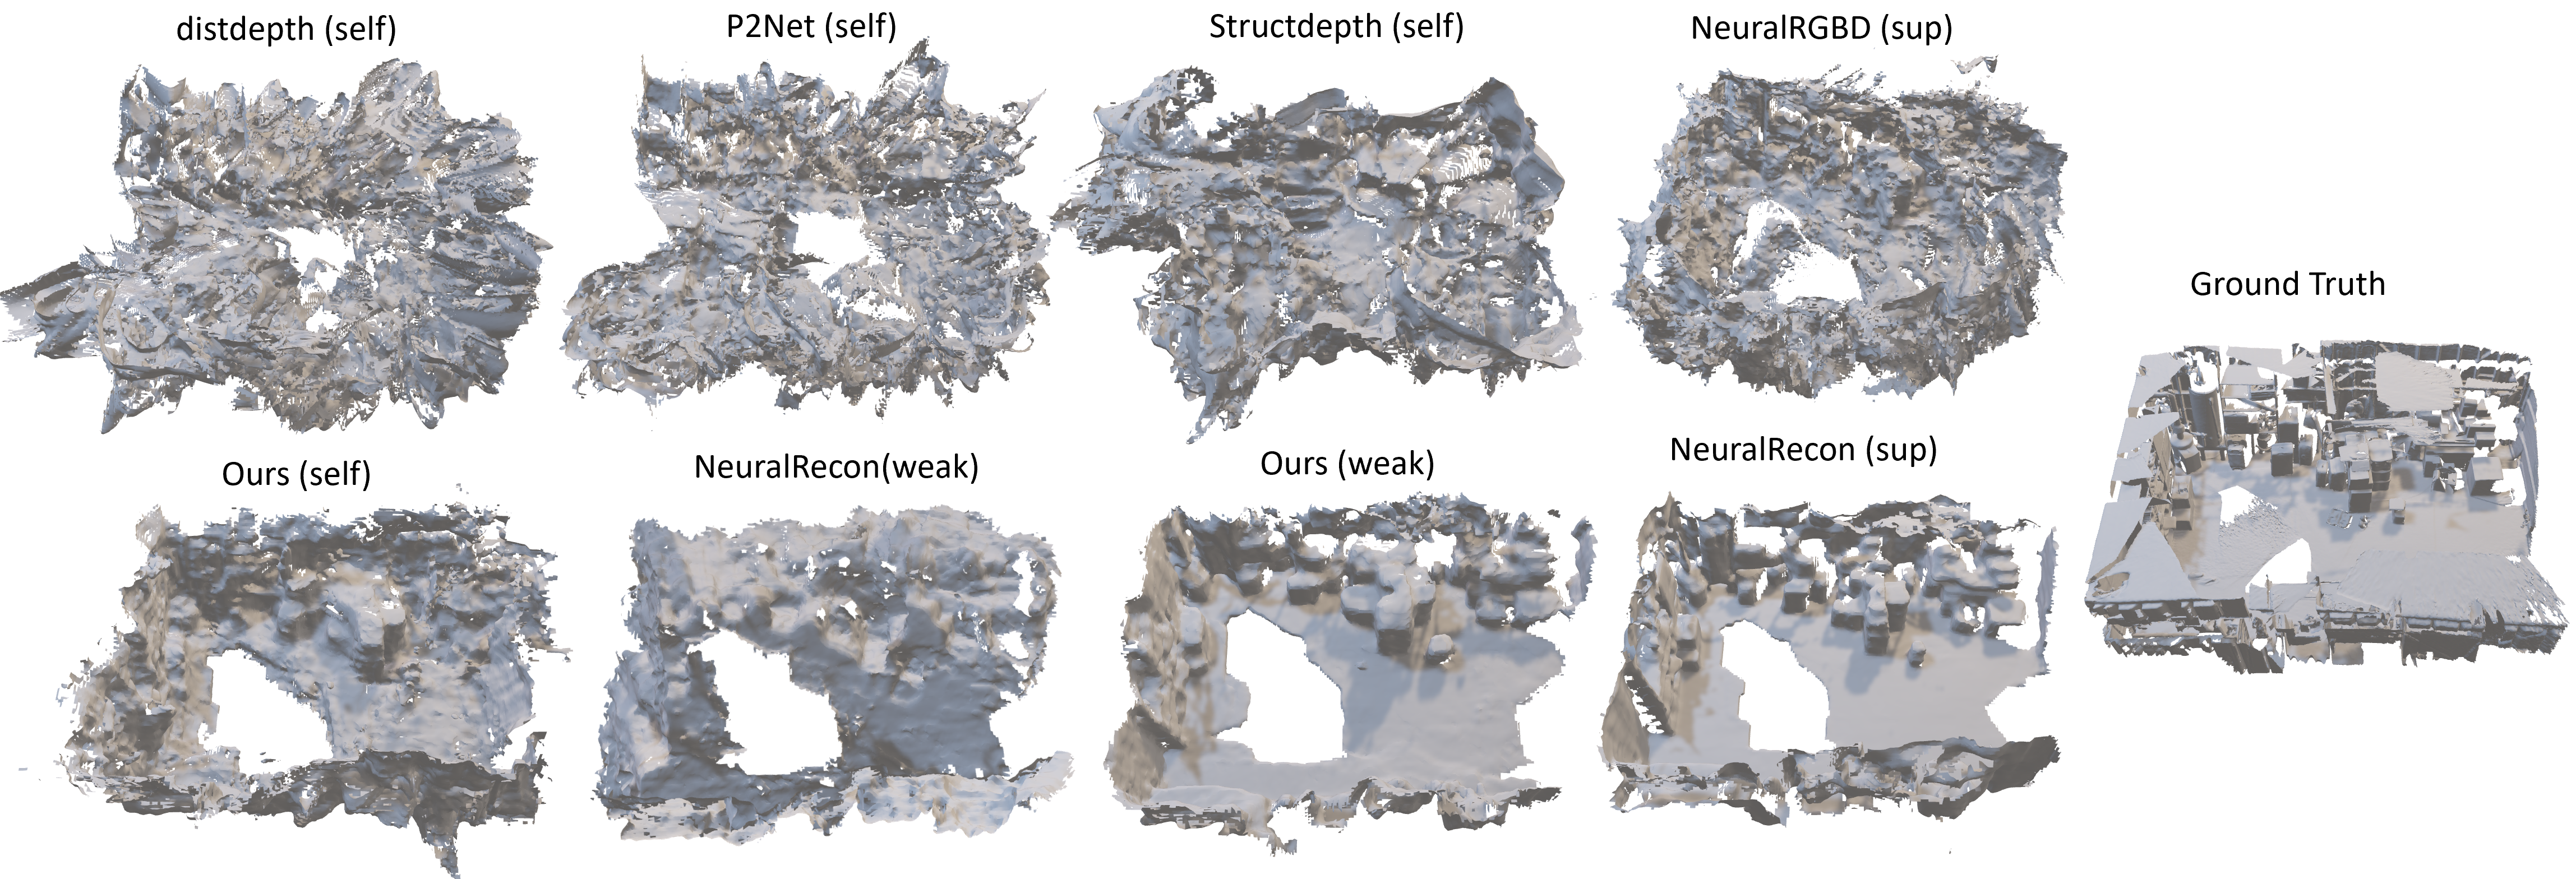
\includegraphics[width=1.0\textwidth]{figures/scannet_mesh/787.png}}
\end{minipage}
\vfill
\begin{minipage}{\linewidth}
  \centerline{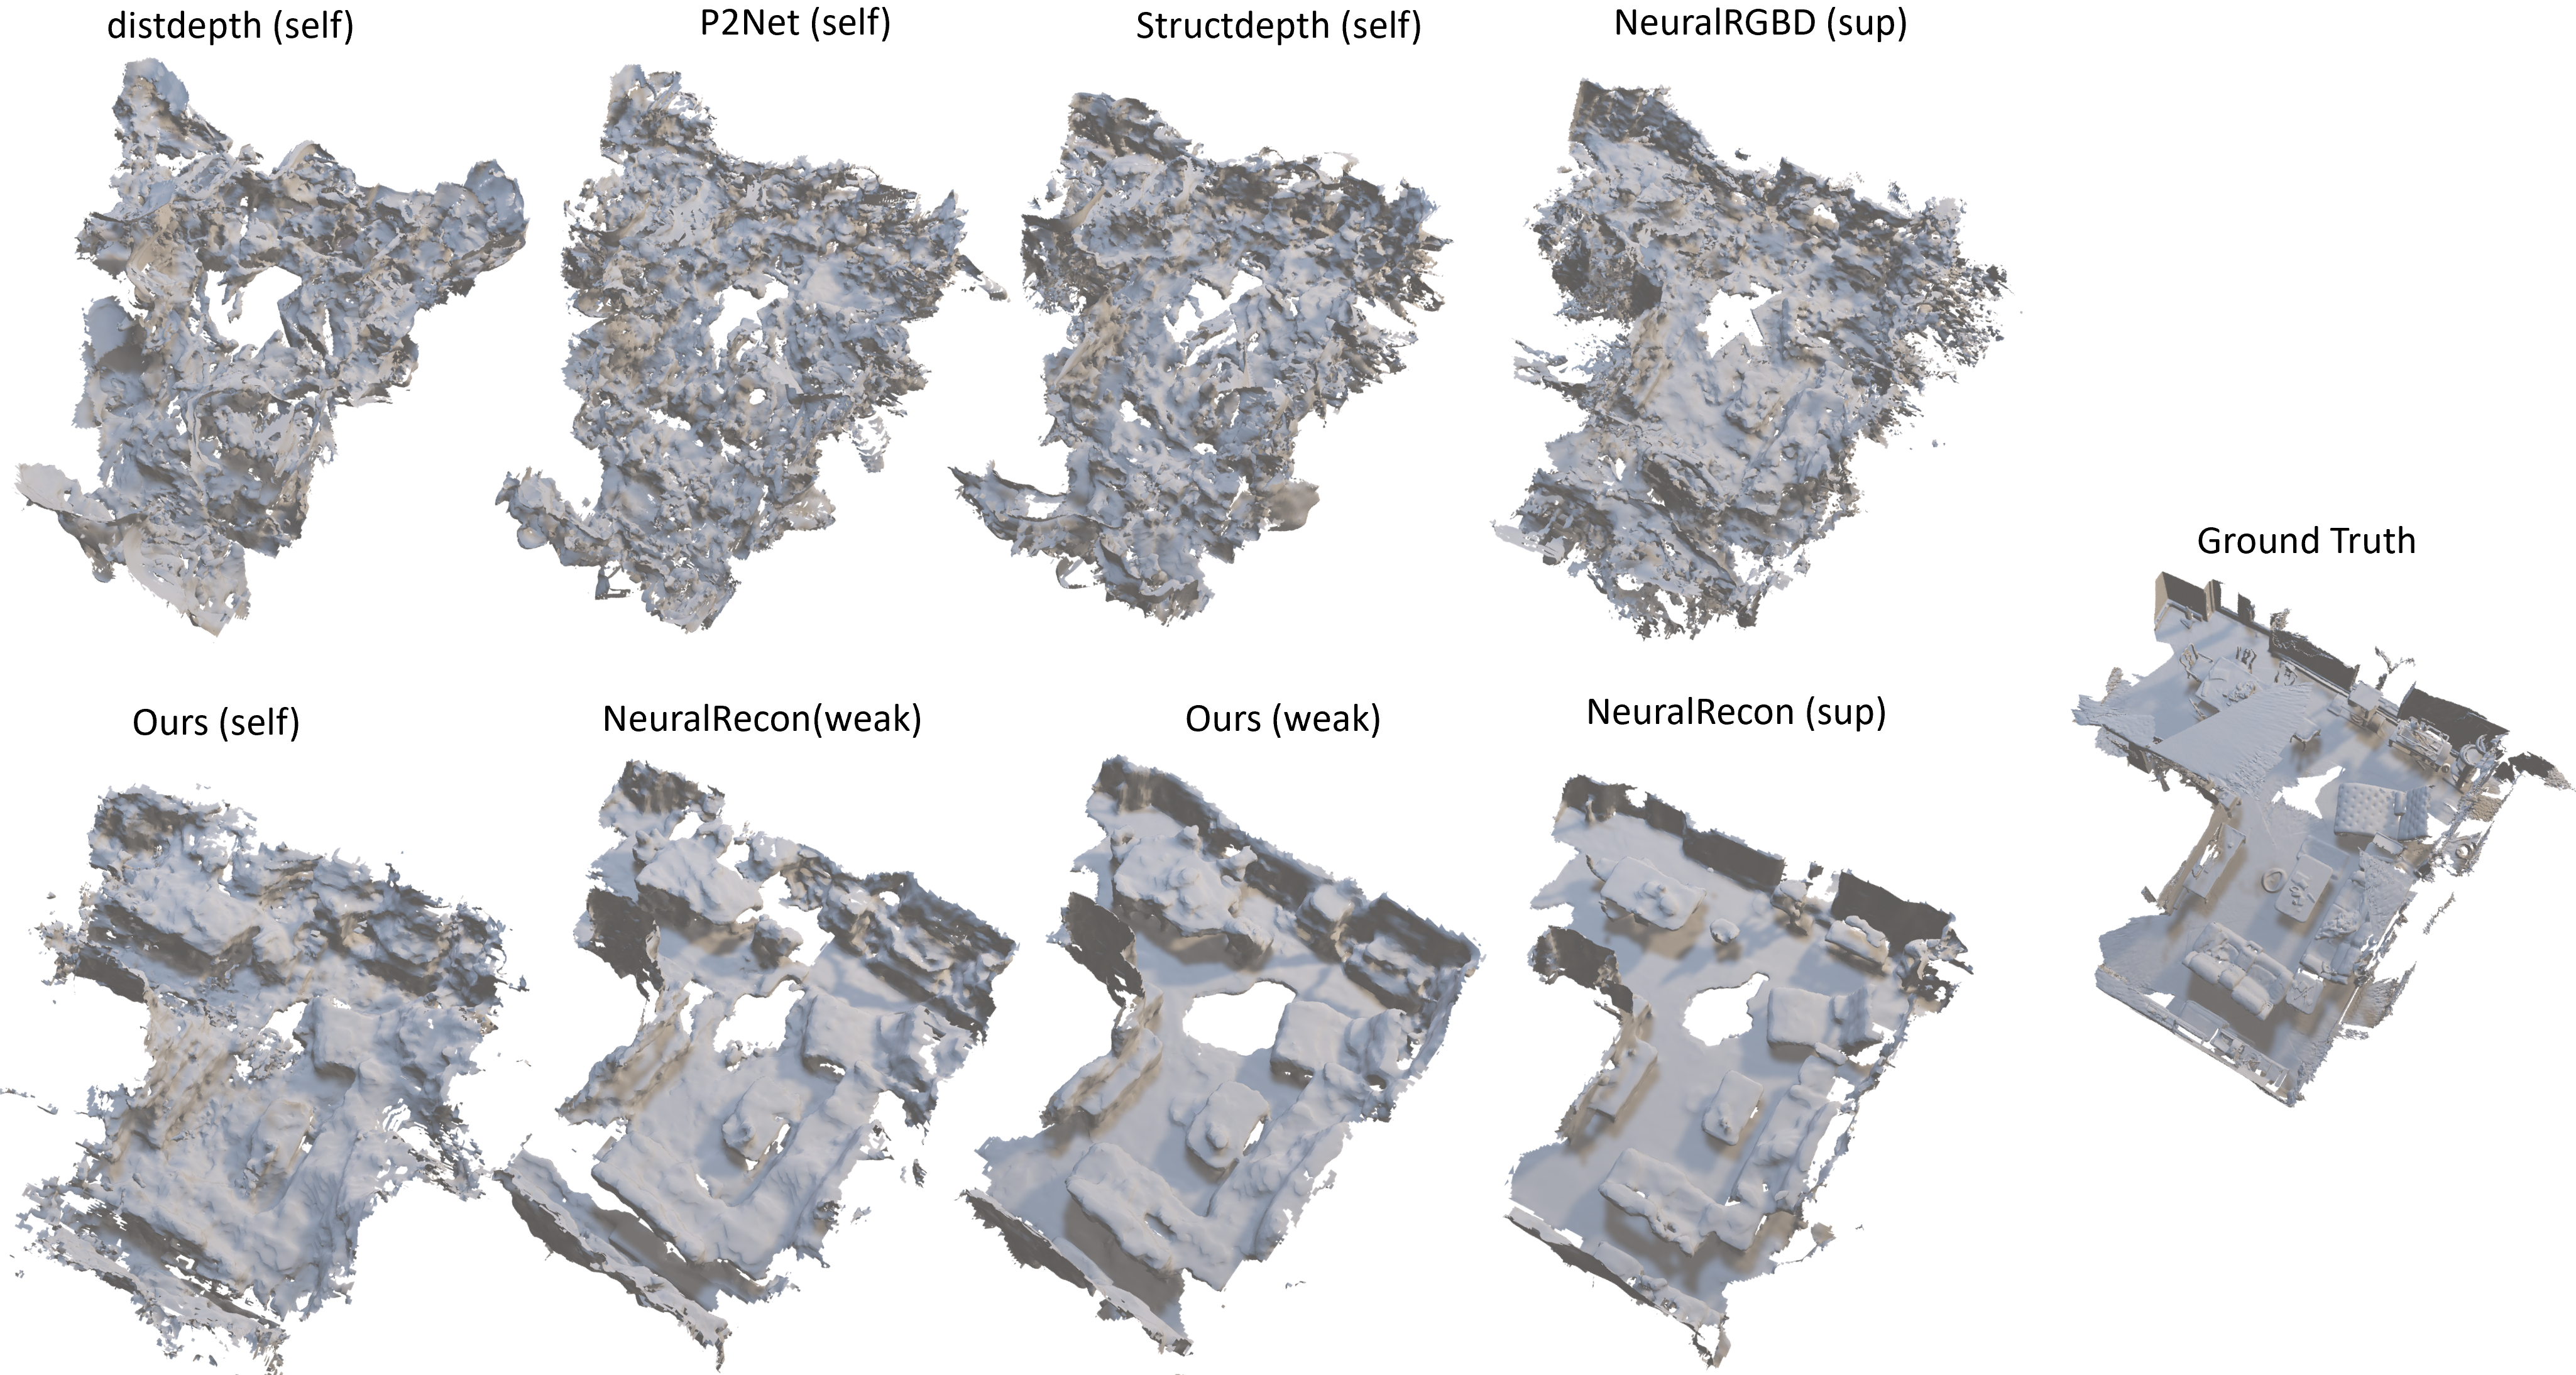
\includegraphics[width=1.0\textwidth]{figures/scannet_mesh/747.png}}
\end{minipage}

\iffalse
\vfill
\begin{minipage}{\linewidth}
  \centerline{\includegraphics[width=1.0\textwidth]{figures/scannet_mesh/710.png}}
\end{minipage}
\fi
\label{fig:scannet_supp}
    \caption{Visual Results}
\end{figure*}


\end{document}
